\paragraph{GET /:lang/user/:userId/search/:keyword/users}
\begin{itemize}
\item \textbf{Successo}
Questo scenario rappresenta il successo di una richiesta che ritorna la lista degli utenti il cui username contiene la keyword inserita nella barra di ricerca che impone, come vincolo per poter essere effettuata, che l'utente sia autenticato al sistema; quindi prima di tale operazione deve venire fatta una richiesta di controllo di sessione mediante l'apposita \textit{REST\ped{G}}. In questo caso il modulo \texttt{UserManagementController} invia \texttt{next()} per indicare il successo dell'operazione.

\begin{figure}[ht]
	\centering
	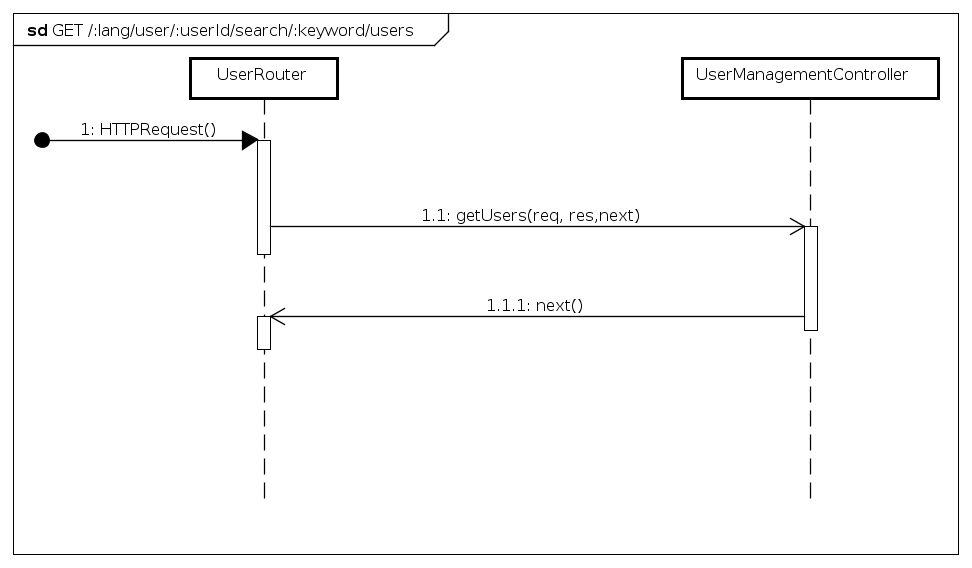
\includegraphics[scale=0.45]{UML/DiagrammiDiSequenza/Back-end/GET__lang_user__userId_search__keyword_users_success.png}
	\caption{Procedura di visualizzazione dei risultati della ricerca utente}
\end{figure}
\FloatBarrier

\item \textbf{Fallimento}
Questo scenario rappresenta il fallimento di una richiesta che ritorna la lista degli utenti il cui username contiene la keyword inserita nella barra di ricerca che impone, come vincolo per poter essere effettuata, che l'utente sia autenticato al sistema; quindi prima di tale operazione deve venire fatta una richiesta di controllo di sessione mediante l'apposita \textit{REST\ped{G}}. In questo caso il modulo \texttt{UserManagementController} invia \texttt{next(error)} per indicare il fallimento di tale vincolo al router il quale avrà compito di reinstradarlo (indirizzandolo verso \texttt{ErrorHandler}).

\begin{figure}[ht]
	\centering
	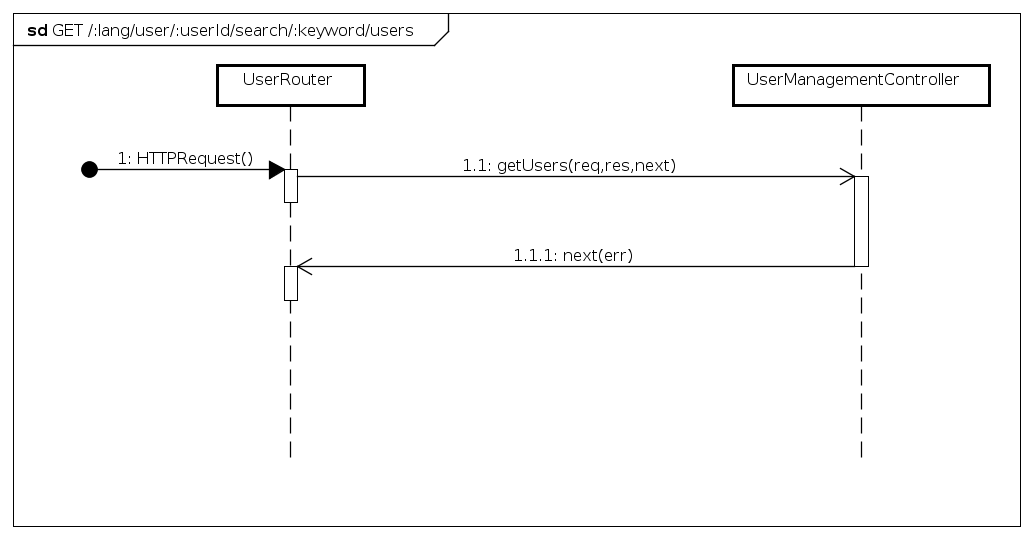
\includegraphics[scale=0.45]{UML/DiagrammiDiSequenza/Back-end/GET__lang_user__userId_search__keyword_users_failure.png}
	\caption{Fallimento della procedura di visualizzazione dei risultati della ricerca utente}
\end{figure}
\FloatBarrier

\end{itemize}






\paragraph{GET /:lang/user/:userId/search/:keyword/quizzes}
\begin{itemize}
\item \textbf{Successo}
Questo scenario rappresenta il successo di una richiesta che ritorna la lista dei questionari il cui titolo contiene la keyword inserita nella barra di ricerca che impone, come vincolo per poter essere effettuata, che l'utente sia autenticato al sistema; quindi prima di tale operazione deve venire fatta una richiesta di controllo di sessione mediante l'apposita \textit{REST\ped{G}}. In questo caso il modulo \texttt{QuizController} invia \texttt{next()} per indicare il successo dell'operazione.

\begin{figure}[ht]
	\centering
	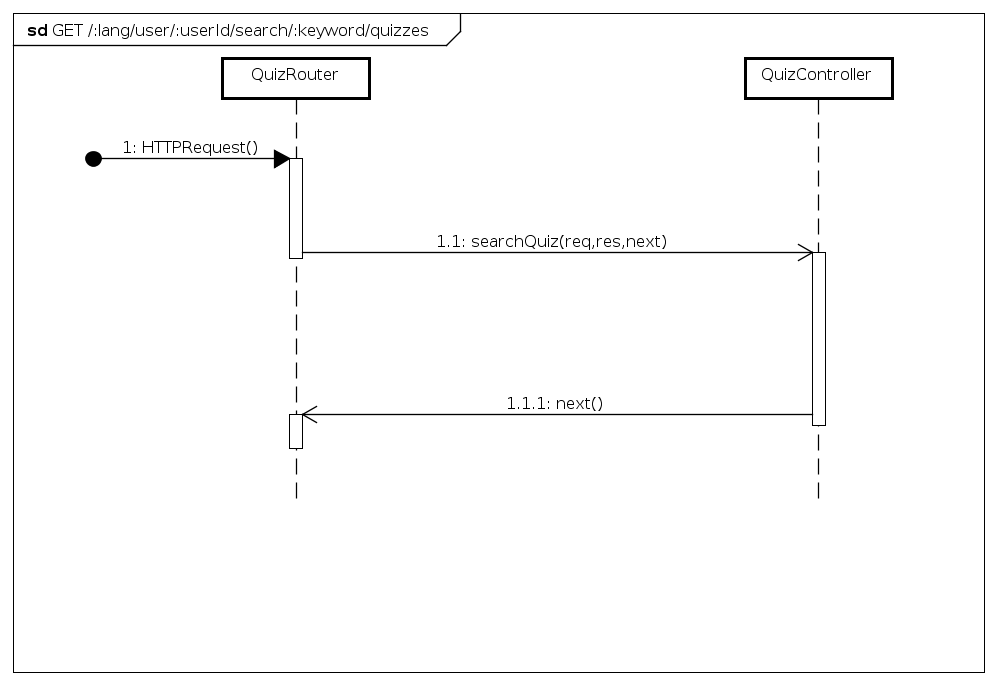
\includegraphics[scale=0.45]{UML/DiagrammiDiSequenza/Back-end/GET__lang_user__userId_search__keyword_quizzes_success.png}
	\caption{Procedura di visualizzazione dei risultati della ricerca questionario}
\end{figure}
\FloatBarrier

\item \textbf{Fallimento}
Questo scenario rappresenta il fallimento di una richiesta che ritorna la lista dei questionari il cui titolo contiene la keyword inserita nella barra di ricerca che impone, come vincolo per poter essere effettuata, che l'utente sia autenticato al sistema; quindi prima di tale operazione deve venire fatta una richiesta di controllo di sessione mediante l'apposita \textit{REST\ped{G}}. In questo caso il modulo \texttt{QuizController} ritornerà un \texttt{next(error)} al router che avrà il compito di reinstradarlo (indirizzandolo verso \texttt{ErrorHandler}).

\begin{figure}[ht]
	\centering
	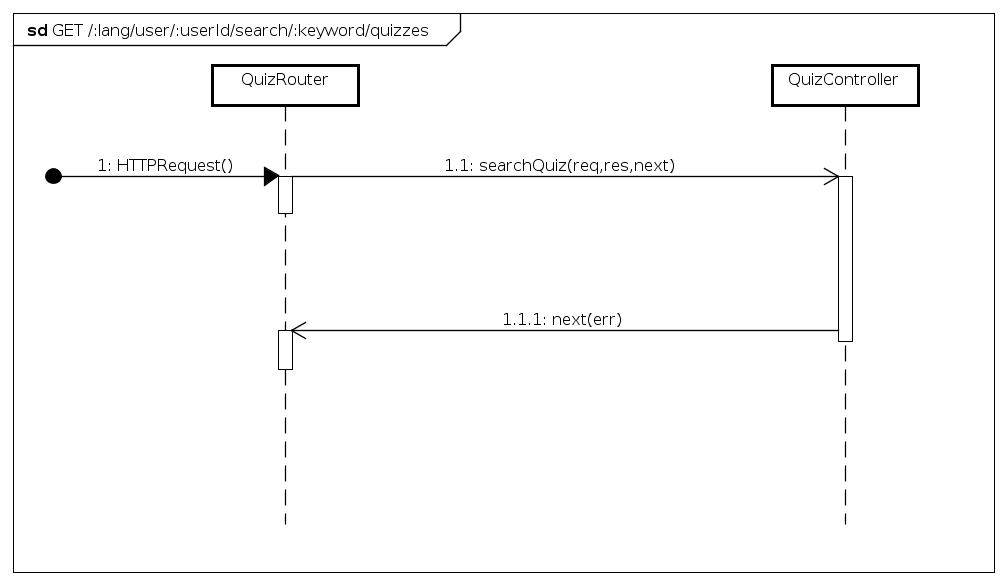
\includegraphics[scale=0.45]{UML/DiagrammiDiSequenza/Back-end/GET__lang_user__userId_search__keyword_quizzes_failure.png}
	\caption{Fallimento della procedura di visualizzazione dei risultati della ricerca questionario}
\end{figure}
\FloatBarrier
\end{itemize}






\paragraph{GET /:lang/user/:userId/search/users/:users}
\begin{itemize}
\item \textbf{Successo}
Questo scenario rappresenta il successo di una richiesta di visualizzazione di un utente tra quelli ritornati come risultato della ricerca che impone, come vincolo per poter essere effettuata, che l'utente sia autenticato al sistema; quindi prima di tale operazione deve venire fatta una richiesta di controllo di sessione mediante l'apposita \textit{REST\ped{G}}. In questo caso il modulo \texttt{UserManagementController} invia \texttt{next()} per indicare il successo dell'operazione.

\begin{figure}[ht]
	\centering
	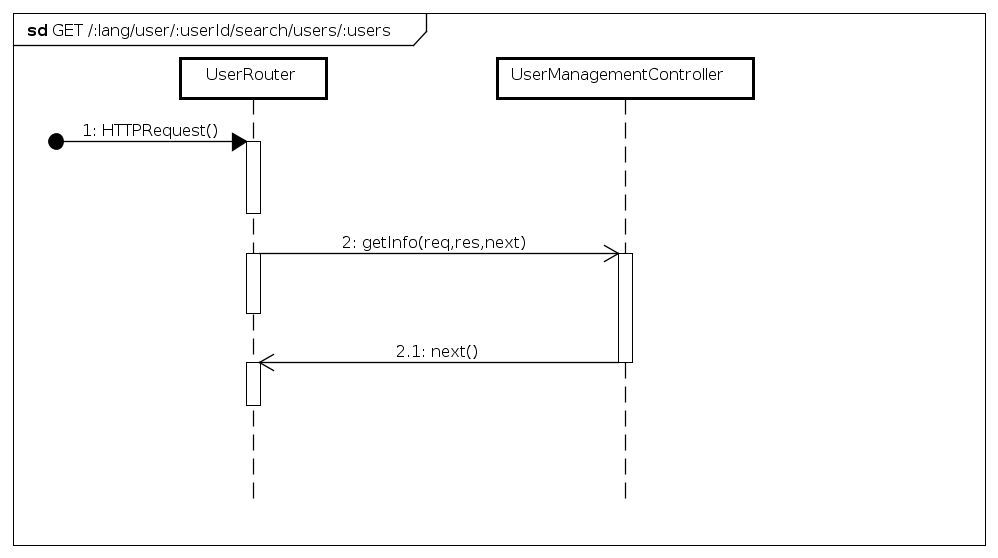
\includegraphics[scale=0.45]{UML/DiagrammiDiSequenza/Back-end/GET__lang_user__userId_search_users__users_success.png}
	\caption{Procedura di visualizzazione di un utente}
\end{figure}
\FloatBarrier

\item \textbf{Fallimento}
Questo scenario rappresenta il fallimento di una richiesta di visualizzazione di un utente tra quelli ritornati come risultato della ricerca che impone, come vincolo per poter essere effettuata, che l'utente sia autenticato al sistema; quindi prima di tale operazione deve venire fatta una richiesta di controllo di sessione mediante l'apposita \textit{REST\ped{G}}. In questo caso il modulo \texttt{UserManagementController} invia \texttt{next(error)} per indicare il fallimento di tale vincolo al router il quale avrà compito di reinstradarlo (indirizzandolo verso \texttt{ErrorHandler}).

\begin{figure}[ht]
	\centering
	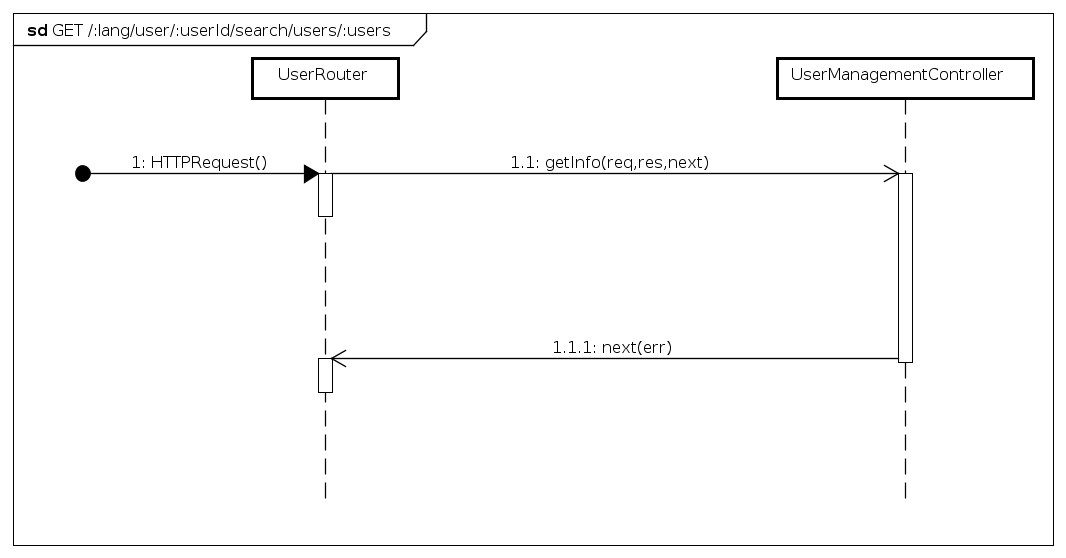
\includegraphics[scale=0.45]{UML/DiagrammiDiSequenza/Back-end/GET__lang_user__userId_search_users__users_failure.png}
	\caption{Fallimento della procedura della visualizzazione di un utente}
\end{figure}
\FloatBarrier

\end{itemize}





\paragraph{GET /:lang/user/:userId/search/quizzes/:quizId}
\begin{itemize}
\item \textbf{Successo}
Questo scenario rappresenta il successo di una richiesta di visualizzazione di un questionario tra quelli ritornati come risultato della ricerca che impone, come vincolo per poter essere effettuata, che l'utente sia autenticato al sistema; quindi prima di tale operazione deve venire fatta una richiesta di controllo di sessione mediante l'apposita \textit{REST\ped{G}}. In questo caso il modulo \texttt{QuizController} invia \texttt{next()} per indicare il successo dell'operazione.

\begin{figure}[ht]
	\centering
	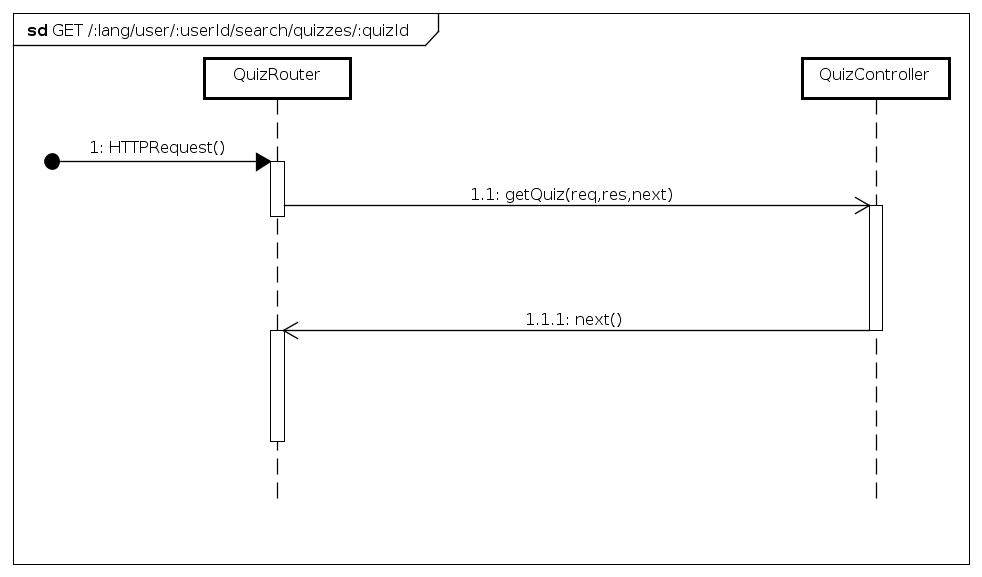
\includegraphics[scale=0.45]{UML/DiagrammiDiSequenza/Back-end/GET__lang_user__userId_search_quizzes__quizId_success.png}
	\caption{Procedura della visualizzazione di un questionario}
\end{figure}
\FloatBarrier

\item \textbf{Fallimento}
Questo scenario rappresenta il fallimento di una richiesta di visualizzazione di un questionario che impone, come vincolo per poter essere effettuata, che l'utente sia autenticato al sistema; quindi prima di tale operazione deve venire fatta una richiesta di controllo di sessione mediante l'apposita \textit{REST\ped{G}}. In questo caso il modulo \texttt{QuizController} ritornerà un \texttt{next(error)} al router che avrà il compito di reinstradarlo (indirizzandolo verso \texttt{ErrorHandler}).

\begin{figure}[ht]
	\centering
	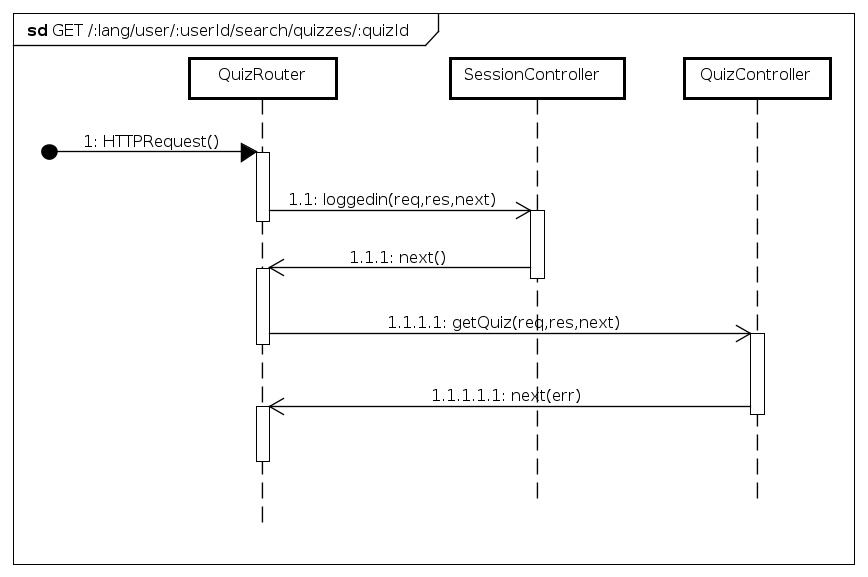
\includegraphics[scale=0.45]{UML/DiagrammiDiSequenza/Back-end/GET__lang_user__userId_search_quizzes__quizId_failure.png}
	\caption{Fallimento della procedura di visualizzazione di un questionario}
\end{figure}
\FloatBarrier

\end{itemize}
